\documentclass[12pt,a4paper,twoside,openright]{report}
\usepackage{preamble} % imported packages/macros/styling from preamble.sty 

\usepackage[sorting=none]{biblatex} % sorting=none means citations in bibliography appear in the order they are cited  
\usepackage[none]{hyphenat} % Disables hyphenation for the entire document. Words will no longer be split across multiple lines with hyphens
\addbibresource{ref.bib} % Add bibliography from ref.bib 

\begin{document}

% TC:ignore tells texcount to ignore word count until TC:endignore 

%TC:ignore

% ----------------------------------------------------------------------

% Title page 
\pagestyle{empty}

\rightline{\LARGE \textbf{\(\langle\)FULL NAME\(\rangle\)}}

\vspace*{30mm}
\begin{center}
	\Huge
	\textbf{\(\langle\)DISSERTATION \\ TITLE\(\rangle\) } \\[20mm]

	\vspace{-2mm}
	
\includegraphics[scale=0.5]{./figures/crest.png}
	\hspace{0mm}\\[20mm]
	\vspace{2mm}


	\LARGE
	Computer Science Tripos -- Part II \\[1mm]
	\(\langle\)COLLEGE\(\rangle\) College \\[20mm]

	\Large
	\today
\end{center}

\newpage
\thispagestyle{empty}

% ----------------------------------------------------------------------

\pagestyle{plain}

\pagenumbering{roman}

% Declaration of originality
\section*{Declaration}

% Check the declaration of originality is up-to-date
I, \(\langle\)FULL NAME\(\rangle\) of \(\langle\)COLLEGE\(\rangle\) College, being a candidate for Part II of the Computer Science Tripos, hereby declare that this dissertation and the work described in it are my own work, unaided except as may be specified below, and that the dissertation does not contain material that has already been used to any substantial extent for a comparable purpose. In preparation of this dissertation I did not use text from AI-assisted platforms generating natural language answers to user queries, including but not limited to ChatGPT. I am content for my dissertation to be made available to the students and staff of the University.

\emph{Signed:} \(\langle\)FULL NAME\(\rangle\)\\
\emph{Date:} \today

% Proforma
\chapter*{Proforma}
 {\large
  \begin{tabular}{ll}
	  Candidate number:   & \(\langle\)CANDIDATE NUMBER\(\rangle\)                                        \\
	  Project Title:      & \bf \(\langle\)DISSERTATION          \\ & \bf TITLE\(\rangle\) \\
	  Examination:        & \bf Computer Science Tripos -- Part II, 2023 \\
	  Word Count:         & \(\langle\)WORD COUNT\(\rangle\)\footnotemark[1]                        \\
	  Code Line Count:    & \(\langle\)LINE COUNT\(\rangle\)\footnotemark[2]                         \\
	  Project Originator: & \(\langle\)PROJECT ORIGINATOR\(\rangle\)         \\
	  Project Supervisor: & \(\langle\)PROJECT SUPERVISOR\(\rangle\)                 \\
  \end{tabular}
 }
\footnotetext[1]{This word count was computed using {\texttt{texcount}}.}
\footnotetext[2]{This code line count was computed using {\texttt{cloc}} (excluding autogenerated test output).}
\stepcounter{footnote}

\section*{Original Aims of the Project}

Lorem ipsum dolor sit amet, consectetur adipiscing elit, sed do eiusmod tempor incididunt ut labore et dolore magna aliqua. Ut enim ad minim veniam, quis nostrud exercitation ullamco laboris nisi ut aliquip ex ea commodo consequat. Duis aute irure dolor in reprehenderit in voluptate velit esse nulla pariatur. Excepteur sint occaecat cupidatat non proident, sunt in culpa qui officia deserunt mollit anim id est laborum.
Fusce ac turpis quis ligula lacinia aliquet. Mauris ipsum. Nulla metus metus, ullamcorper vel, tincidunt sed, euismod in, nibh.

\section*{Work Completed}

Lorem ipsum dolor sit amet, consectetur adipiscing elit, sed do eiusmod tempor incididunt ut labore et dolore magna aliqua. Ut enim ad minim veniam, quis nostrud exercitation ullamco laboris nisi ut aliquip ex ea commodo consequat. Duis aute irure dolor in reprehenderit in voluptate velit esse nulla pariatur. Excepteur sint occaecat cupidatat non proident, sunt in culpa qui officia deserunt mollit anim id est laborum.
Fusce ac turpis quis ligula lacinia aliquet. Mauris ipsum. Nulla metus metus, ullamcorper vel, tincidunt sed, euismod in, nibh.

\section*{Special Difficulties}

None.

\newpage 

% Table of contents 
\tableofcontents


% ----------------------------------------------------------------------
\newpage
\pagenumbering{arabic}
\setcounter{page}{1}
%TC:endignore

% textcount's word count is now enabled 


% Remove code snippets and algorithms from word count 
%TC:envir minted 1 xall 
%TC:macro \mintinline [ignore]
%TC:envir algorithmic 1 xall

% Include tables in word count
%TC:envir table 0 word
%TC:envir tabular 1 word

% Include footnotes in word count
%TC:macro \footnote [text]
%TC:macro \footnotetext [text]


% Main chapters
\addtocontents{lol}{\protect\vspace*{10pt}}
\chapter{Introduction}
% Well-motivated project with success criteria well-justified.

\label{sec:introduction}
Visual Simultaneous Localization and Mapping (visual SLAM) serves as the foundation of countless modern technologies, with self-driving cars, augmented reality devices, and autonomous drones just being a few examples. By using purely visual inputs, visual SLAM is able to create a 3D map of the surroundings while also localizing the camera's position within this map in real-time.

Unlike other SLAM systems which may use an expensive and heavy sensor such as LIDAR, RGB-Depth cameras, or Radar, visual SLAM only requires the ubiquitous camera sensor, allowing the technology to be used in many commercial applications such as Google's ARCore\footnote[1]{\url{https://developers.google.com/ar/develop/fundamentals}}, Boston Dynamic's GraphNav system used on their robot Spot\footnote[2]{\url{https://support.bostondynamics.com/s/article/GraphNav-Technical-Summary}}, and several models of DJI quadcopters\footnote[3]{DOI: 10.1016/j.vrih.2019.09.002} making this a particularly practical field of research.

\section{Motivation}
\label{sec:motivation}
Multi-robot systems are becoming increasingly common as automation continues to grow in a variety of fields, such as self-driving cars, drone swarms, and warehouse robots. These systems require the agents to understand the world around them as well as their peer's locations within that world. This task is often achieved with technologies such as GPS or motion capture setups, however, not all environments have access to these systems. A few emerging examples include: \noparskip
\smallbreak

{
    \begin{itemize}[nosep]
        \item Search and rescue operations in large indoor systems, assisted by drone swarms.
        \item Self-driving cars in underground road networks.
        \item Multi-agent cave/subsea exploration.
    \end{itemize}
}

These are scenarios where multi-agent SLAM provides a compelling solution, as it enables us to build a map of an unknown environment and keep agents aware of their relative poses. However, the majority of existing multi-agent visual SLAM implementations are centralized systems, requiring the agents to maintain reliable communications with a central server in order to operate. This is extremely detrimental, as environments that do not have access to GPS or motion capture systems are also likely to have very poor communication channels – greatly limiting the use cases of these centralized multi-agent SLAM systems.

Naturally, this leaves us with distributed multi-agent visual SLAM systems that do not rely on a centralized management server, allowing the agents to be used in environments where network infrastructure may be lacking. Instead of a central node, the agents are able to communicate peer-to-peer when they come within close proximity to one another.

It is easy to see the broad-reaching use cases of such a system. Agents will be able to explore sections of the world independently or in small teams, sharing new world locations with their peers as they come into communication range using an ad-hoc network. Agents will be able to accurately determine their peer's locations when they are within communication range, allowing for collision avoidance and cooperative path planning.

\section{Project Overview}
\label{sec:project-overview}
In this project, I: \noparskip
{
    \begin{enumerate}
        \item \textbf{Design and implement the first distributed monocular visual SLAM system available.} \comment{how do I ensure it really is the first?} It is capable of localization, relative pose estimation, and collaborative mapping, all while being tolerant to degraded network conditions and not reliant on any single leader agent. % TODO: talk about my "novel" DPGO approach?
        \item Evaluate the performance of my system on standardized datasets, \textbf{demonstrating its superior performance over comparable state-of-the-art systems}.
        \item Create a simulation environment for testing and evaluating my system locally.
        \item Deploy my system on physical robots, \textbf{demonstrating the practical use cases of this system and benchmarking real-world performance.} Additionally, \textbf{I was an author of the paper \textit{The Cambridge RoboMaster: An Agile Multi-Robot Research Platform}}, with my distributed SLAM system included as one of the experiments analyzed in the paper.
        \item Develop \textit{Multi-Agent EVO} – the first open-source evaluation library for multi-agent SLAM systems.
        \item Develop the \textit{Raspberry Pi Video Publisher} – a performant platform for SLAM data collection or augmented reality visualizations – and set up a continuous integration and deployment pipeline to automatically push the latest build to the hardware.
    \end{enumerate}
}

\begin{leftbar}
    \textbf{A short video demonstration of my project is provided at the following URL:} \url{https://cam-diss.s3.amazonaws.com/video.mp4} \comment{TODO: fix video index}

    Due to the highly visual and 3D nature of my project, \textbf{I strongly recommend viewing the video}. It will provide an intuition of my system, making the following chapters easier to visualize and understand. Additionally, it is referenced throughout the dissertation.
\end{leftbar}

\begin{figure}[h]
    \centering
    \captionsetup{format=plain}
    \begin{subfigure}[t]{0.475\linewidth}
        \centering
        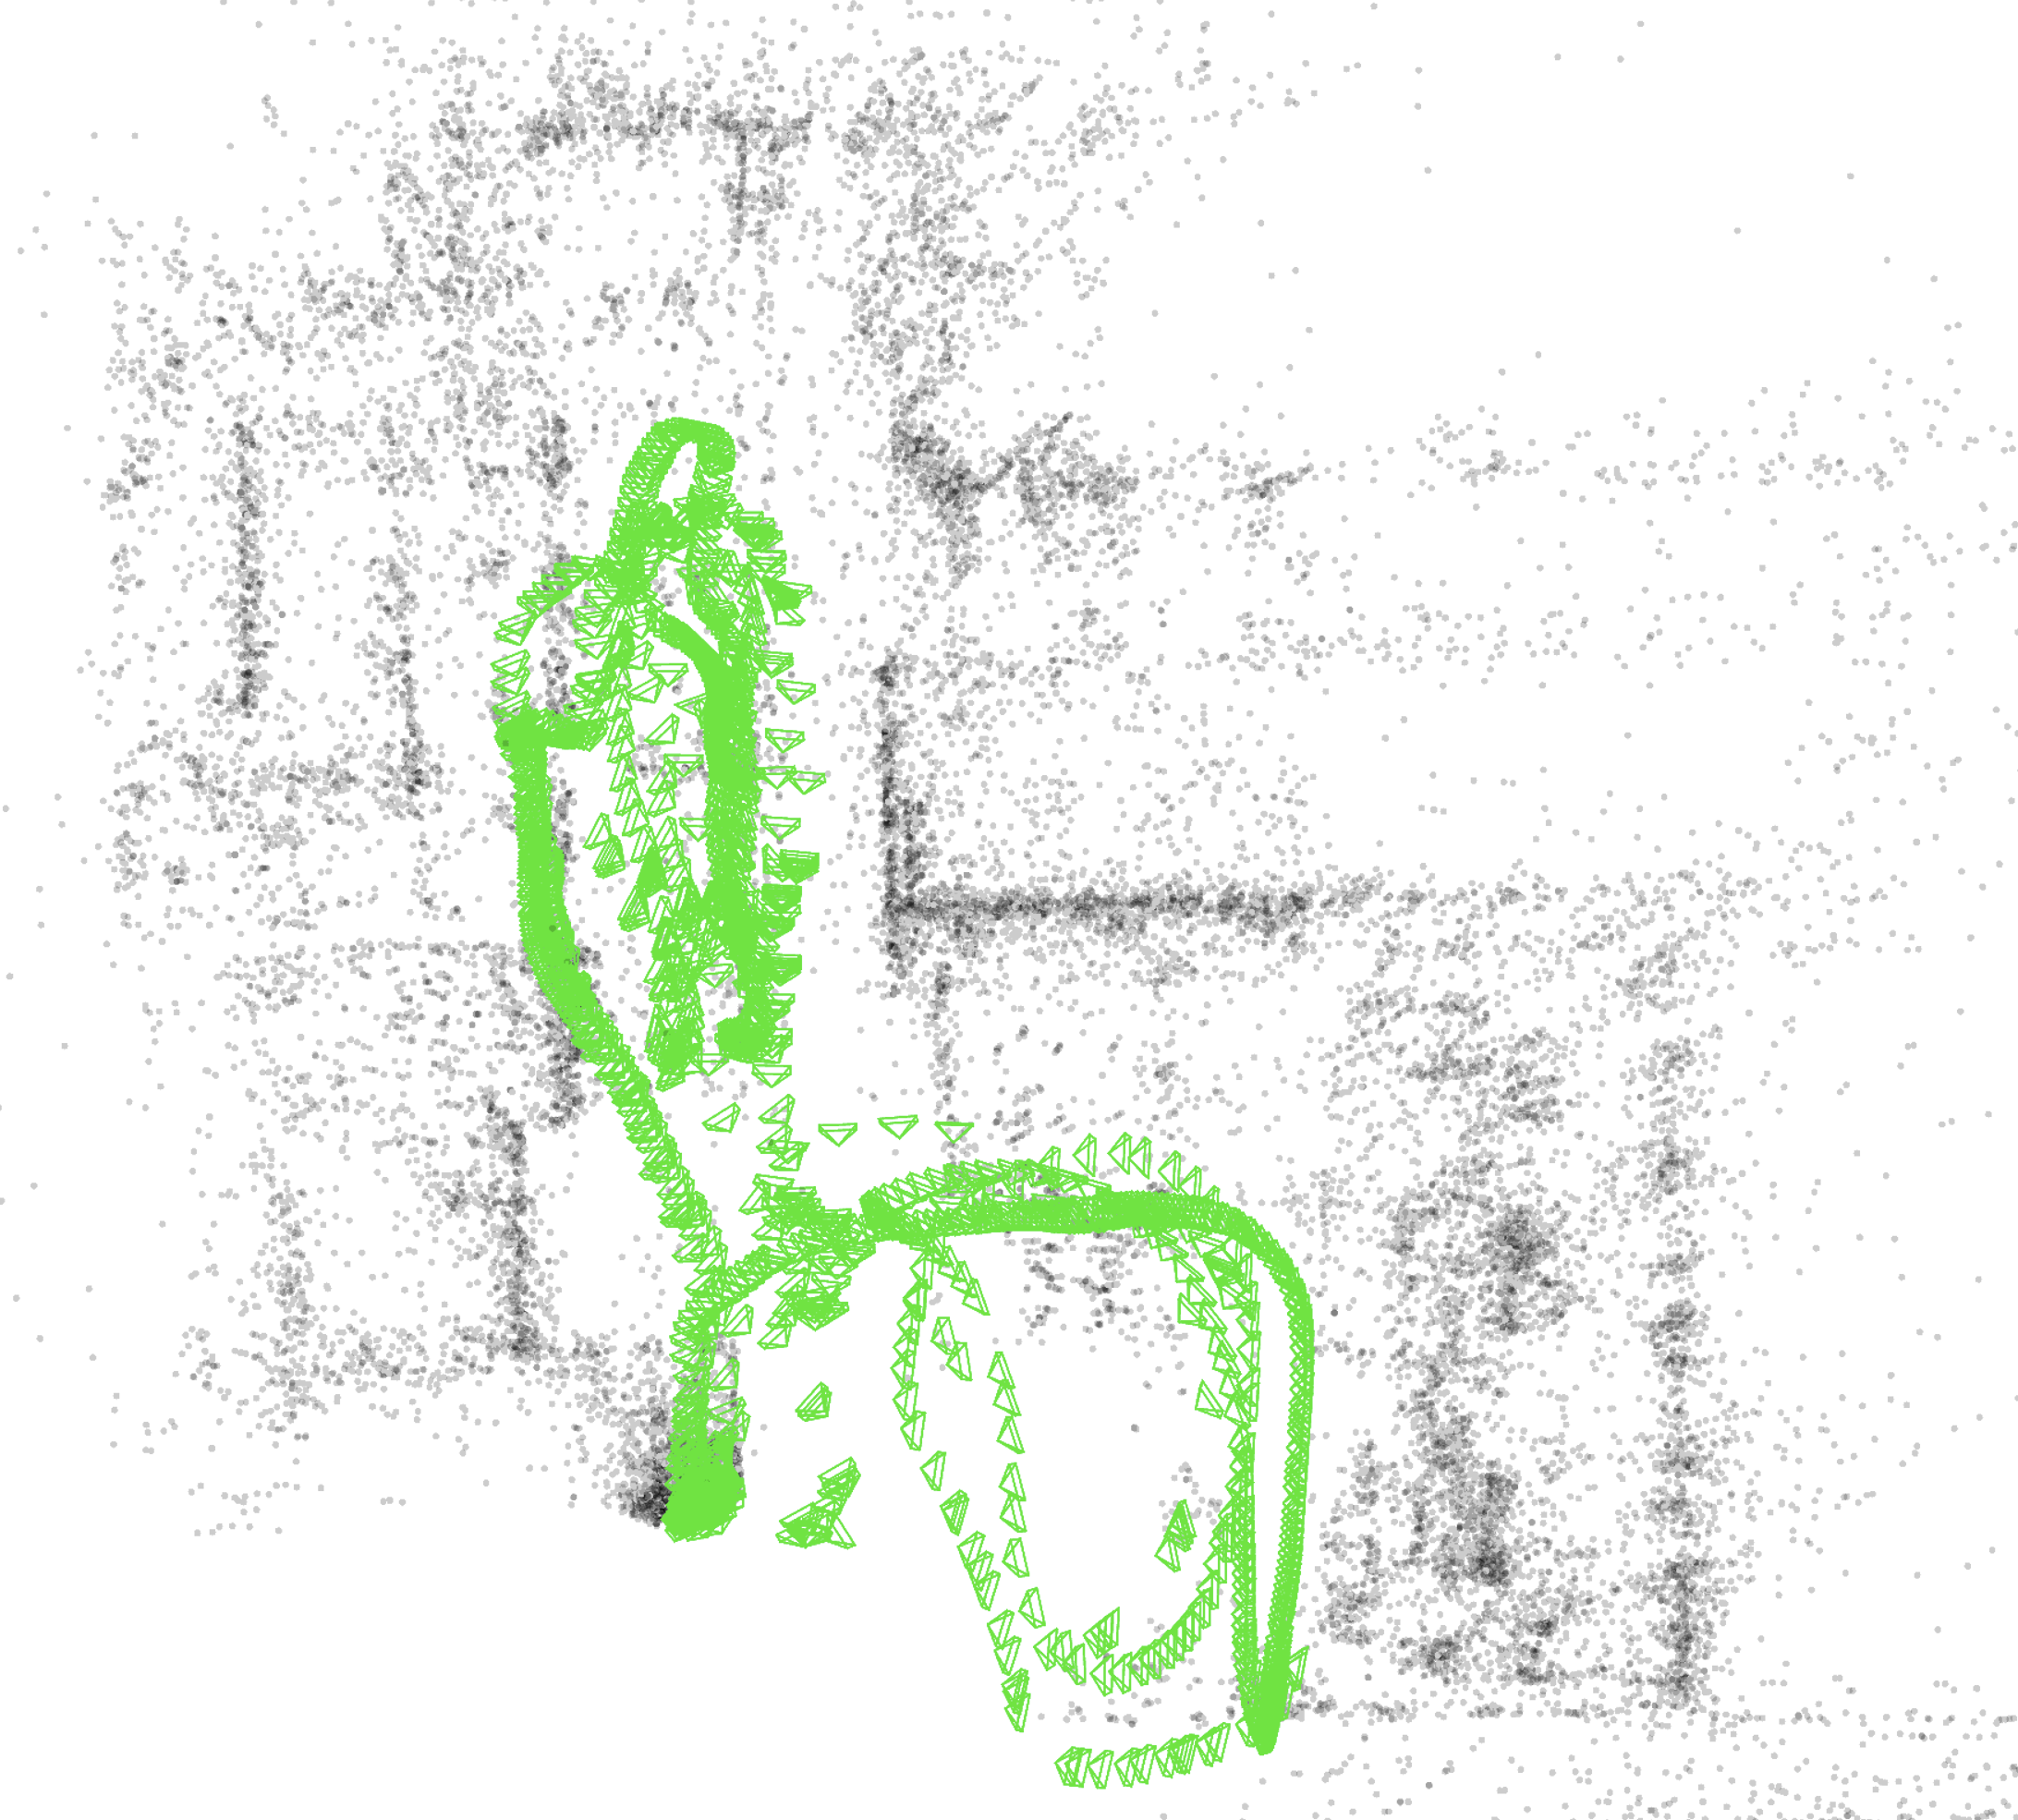
\includegraphics[height=2.4in]{figures/euroc_mh_map.png}
        \caption{EuRoC Machine Hall 01-03}
    \end{subfigure}\hfill%
    ~
    \begin{subfigure}[t]{0.475\linewidth}
        \centering
        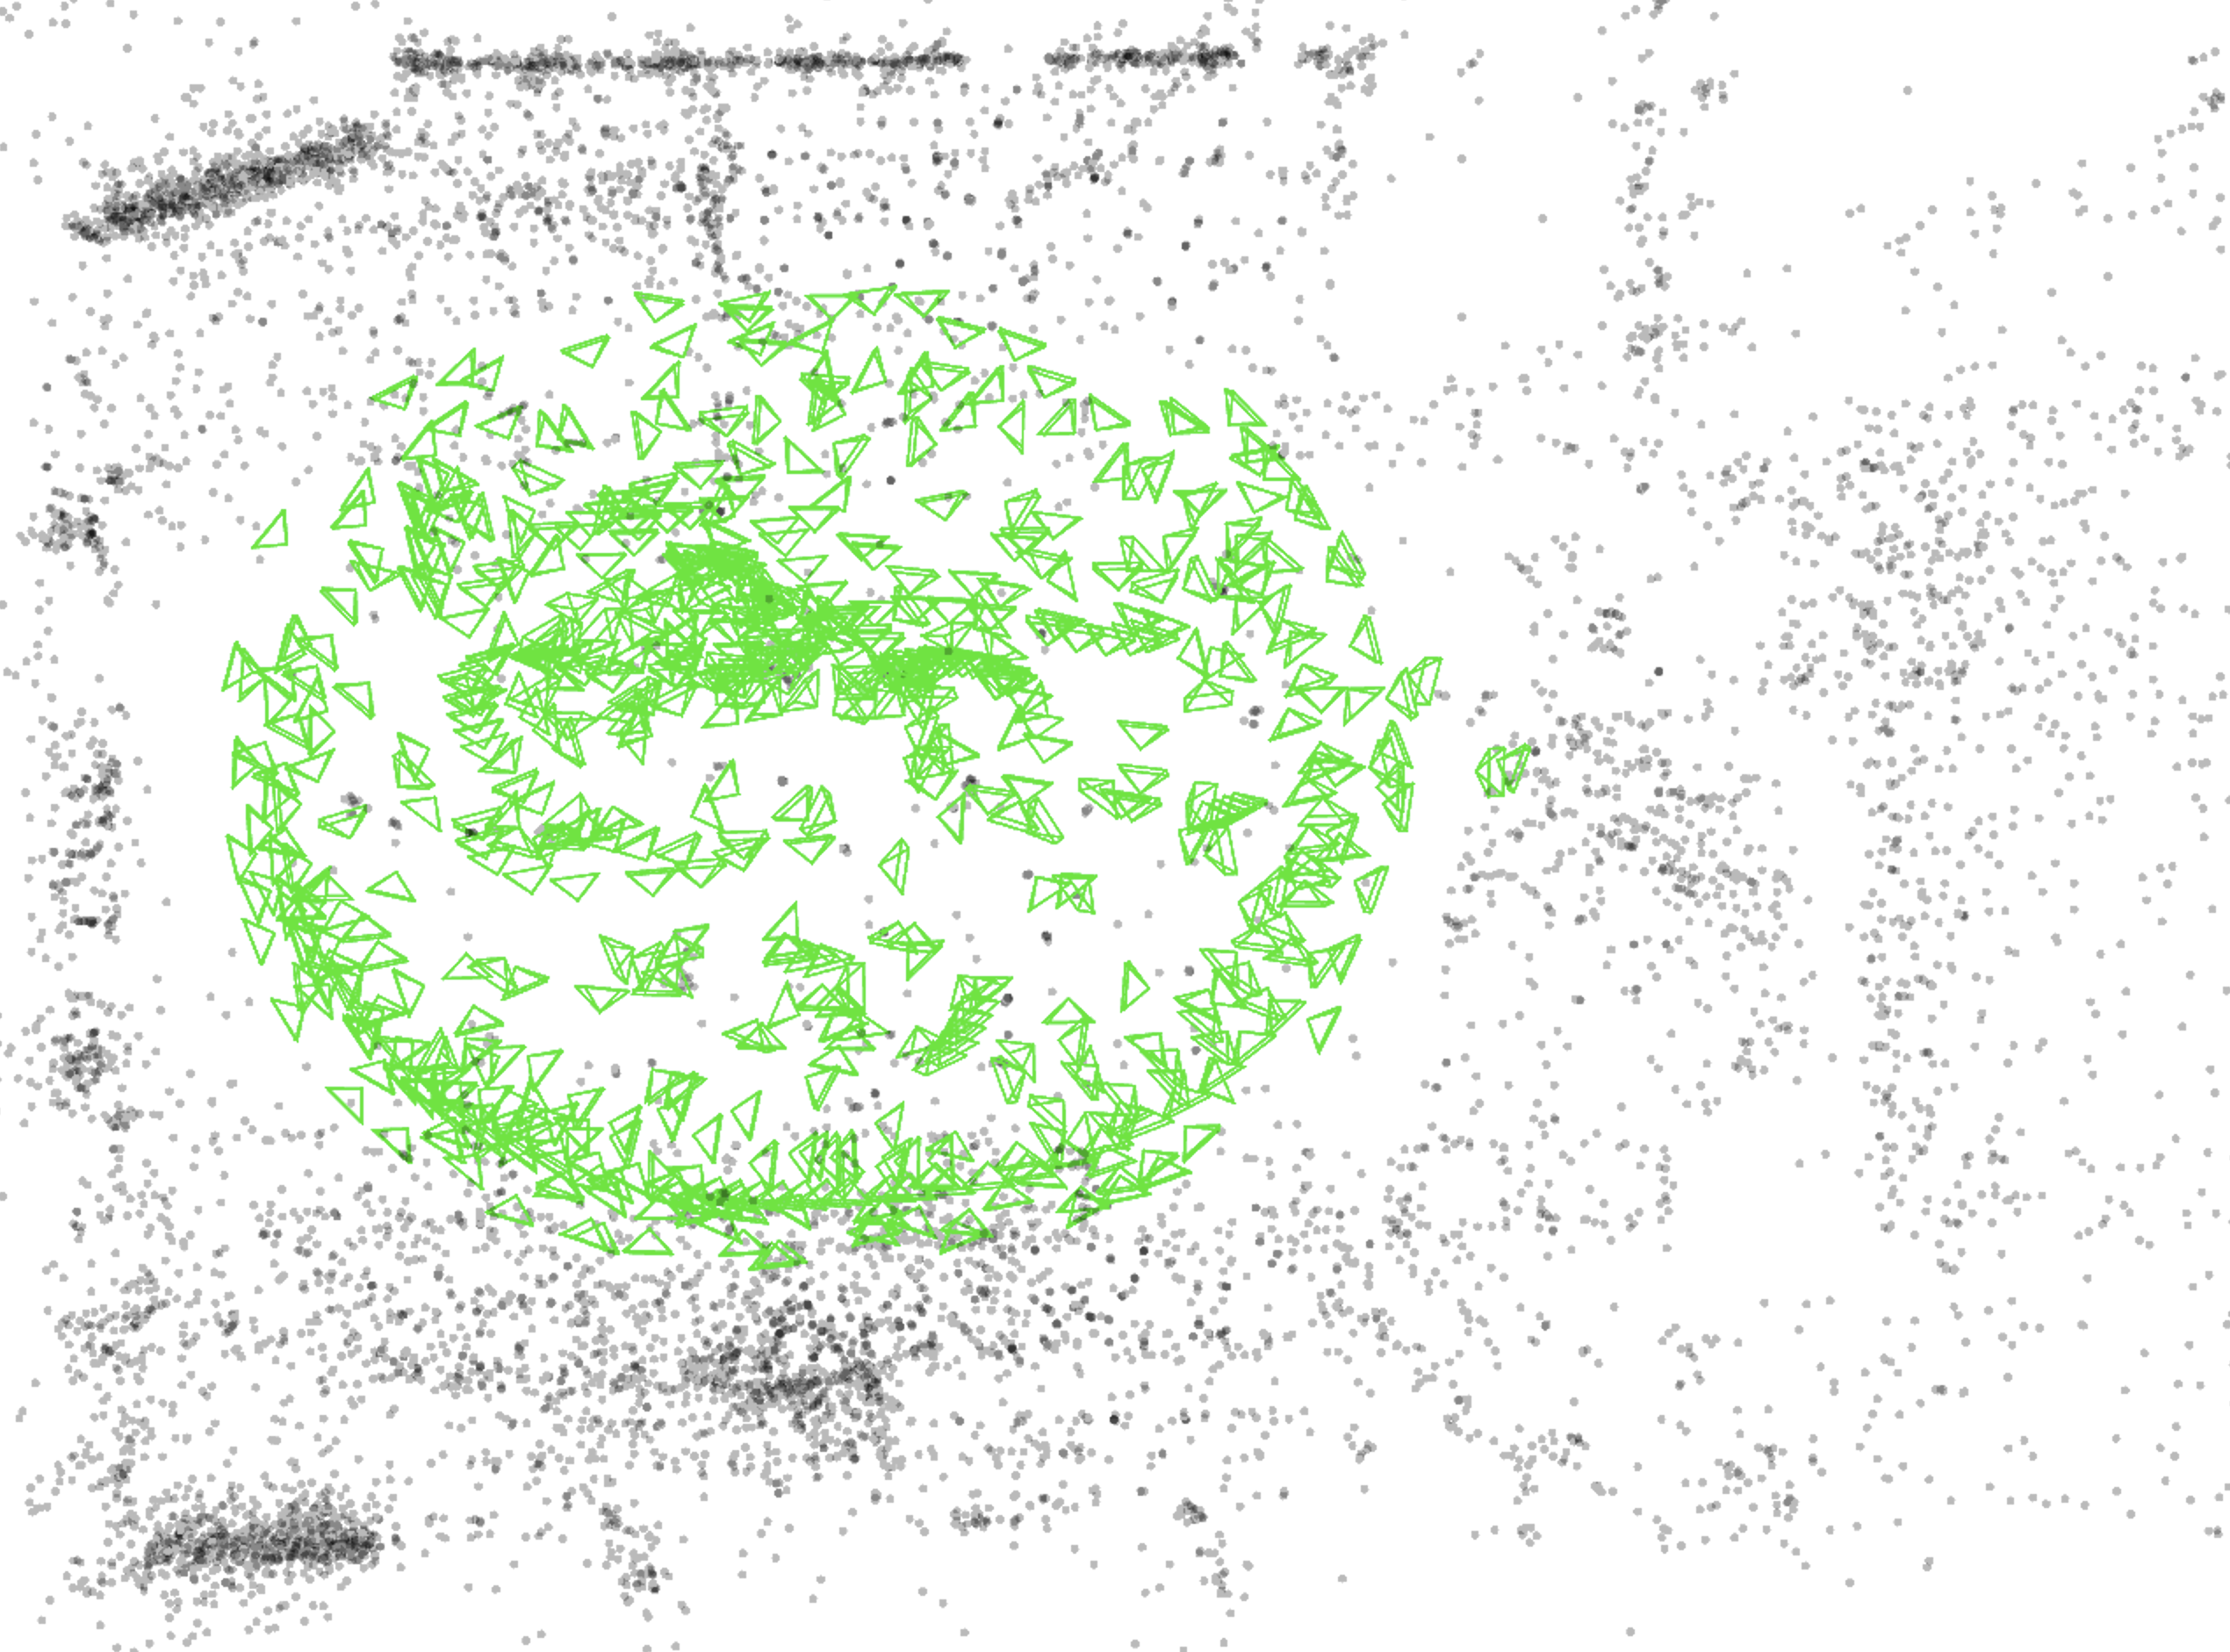
\includegraphics[height=2.2in]{figures/tum_room_map.png}
        \caption{TUM-VI Rooms 1-3}
    \end{subfigure}

    \caption{Sparse maps built by my distributed SLAM system running industry-standard datasets.}
    \label{fig:example-maps}
\end{figure}


\addtocontents{lol}{\protect\vspace*{10pt}}
\chapter{Preparation}
% it is essential to demonstrate that a proper professional approach was employed

% It should show how the project proposal was further refined and clarified, so that the implementation stage could go smoothly rather than by trial and error.

% You must demonstrate a structured design approach, including high-level design planning, design-for-test, consideration of human factors and systematic evaluation including confidence metrics within your evaluation where appropriate. You should explain how you would show conformance with appropriate legislation, such as that for intellectual property, data protection, human subjects and software licenses such as those for open source. Show that you understand the consequences of your project (or a more fully-formed variant of it) in terms of how it might affect commercial markets, contribute to society and/or the research community.

% Challenging and well-presented background covering Comp Sci topics beyond Part IB.

% Good requirements analysis, justified selection of suitable tools, good engineering approach.

\label{sec:2}

\section{Starting Point}
\label{sec:starting-point}
As noted in the \hyperref[sec:relevant-work]{\textit{Relevant Work}} section, visual SLAM systems are a mature and well-researched subfield of Computer Science with many advanced implementations. To avoid spending the majority of my effort re-implementing a visual SLAM system from scratch, I instead used a \textbf{single-agent} visual SLAM implementation as the starting point for my project. The thinking behind this decision was that it would allow me to focus my efforts on the distributed multi-agent aspect of this project, which I believe is a novel and under-researched aspect of the field.

I chose ORB-SLAM3 as the single agent SLAM system to base my system on top of, as it ranks at the top of benchmarks in a variety of environments \autocite{DBLP:journals/corr/abs-2108-01654} and its researchers released code alongside their paper. I primarily utilized the system's visual odometry (VO) front end and helper functions from the backend to perform operations such as bundle adjustment.

While ORB-SLAM3 is an excellent SLAM system, it is fundamentally a single-agent system with no considerations in place for use in a multi-agent context. As I will expand on in the \hyperref[sec:orb-slam-3]{\textit{ORB-SLAM 3}} section, a significant amount of time and effort was required to understand its extremely large undocumented codebase, especially since an almost complete understanding of its inner workings were needed to both extract and inject map information from the system. In retrospect, using an existing single-agent SLAM system as a foundation may not have saved as much time as I had initially hoped.

Nevertheless, using a cutting-edge single-agent SLAM system as a foundation for my project has allowed me to create a distributed SLAM system that is accurate and performant enough to have real-world use cases.

At the time of submitting my project proposal, I had forked the ORB-SLAM3 \autocite{ORBSLAM3_TRO} git repository\footnotemark[1] and explored the codebase. ORB-SLAM3 is licensed under GPL-3.0, and as such, I have open-sourced my code under the same license\footnotemark[2].

\footnotetext[1]{\url{https://github.com/UZ-SLAMLab/ORB_SLAM3}}
\footnotetext[2]{\url{https://github.com/jyjblrd/part_II_project} TODO: Redact}

I had no prior experience working with SLAM systems, but I had researched the current state of multi-agent visual SLAM systems to evaluate the feasibility of my project and to prevent it from being a duplication of prior work.

\section{Relevant Work}
\label{sec:relevant-work}
While single-agent SLAM systems are a relatively mature field of research, multi-agent systems are still very much in active development.


TODO: move to PGO section?
Pose Graph Optimization (PGO) is the backbone of many modern SLAM systems, and is essential to understanding how multi-agent systems operate. PGO is an optimization method, which represents agent poses and landmarks as nodes on a graph and constraints as edges between these nodes. For example, if a pose observes a landmark there will be a constraint (represented by a cost function) describing the landmark's location relative to the pose. PGO works by optimizing this graph, optimizing the pose and landmark locations to best satisfy the constraints.

Centralized multi-agent systems such as CCM-SLAM(2019) \autocite{schmuck2019ccm} and COVINS(2021) \autocite{schmuck2021covins} require a centralized server to perform map merges and PGO. While simpler to implement, this comes with the obvious limitations that come with centralized systems such as scalability issues and requiring existing networking infrastructure.

In recent years we have seen the emergence of a handful of decentralized multi-agent systems, however they have various limitations. Various systems such as \autocite{doi:10.1126/scirobotics.abm5954} \autocite{8658783} \autocite{DBLP:journals/corr/abs-2103-12770} require the agents to be initialized with their ground truth poses, which limits their real-world usability. In contrast, my system is able to provide accurate relative localization even when agents are initialized in arbitrary and unknown locations by identifying common landmarks in the world.

Table TODO lays out the sensor configurations used by other various state-of-the-art distributed SLAM systems, showing that my system stands out as the only one capable of operating with purely monocular visual data. This is advantageous, as LiDAR \& RGBD sensors have considerable weight, and stereo cameras may require a minimum camera separation to operate, both of which limit their usage on small aerial robots.


TODO: fact check below lol
Additionally, my system provides a novel approach to the Distributed Pose Graph Optimization (DPGO) problem. There are various methods to approaching DPGO. SWARM-SLAM(2024) \autocite{Lajoie_2024} elects a single agent to perform the PGO for the entire swarm, which is simple but has a high communication overhead since all agents have to send their pose estimations before each optimization. Other systems perform DPGO by spreading computation across agents by using algorithms such as ARock \autocite{Peng_2016} or Distributed Gauss-Seidel \autocite{DBLP:journals/corr/ChoudharyCNRCD17}, however these methods still present a communication overhead and may stall under unreliable communication.

Instead of performing discrete optimization runs, my method of DPGO is performed incrementally. Each agent optimizes its pose graph as external data streams in, with an additional map alignment step performed on a timer. This method has no additional communication overhead, apart from the infrequent map alignment step, and we analyze its performance in the \nameref{sec:benchmarking} Section. The details of this are presented in the \nameref{sec:decentralized-system-manager} Section.


% DOOR-SLAM(2020) \autocite{Lajoie2020DOORSLAM} uses the Distributed Gauss-Seidel approach to Distributed Pose Graph Optimization (DPGO) proposed by Choudhary et al. in 2017 \autocite{DBLP:journals/corr/ChoudharyCNRCD17} while Kimera-Multi(2022) \autocite{tian22tro_kimeramulti} utilizes distributed graduated non-convexity for DPGO. However,

% Xu et al. \autocite{xu2022d} argue that DOOR-SLAM(2020) \autocite{Lajoie2020DOORSLAM} and Kimera-Multi(2022)'s distributed pose graph optimization methods prevent their systems from achieving accurate relative localization. $D^2$SLAM(2022)'s \autocite{xu2022d} near field and far field estimation systems allow it to achieve accurate relative localization while maintaining global consistency, however it

% often use some method of distributed optimization to refine the shared map. Most commonly this is done using Distributed Pose Graph Optimization (DPGO), which globally optimizes the shared map, providing good global consistency but often lacking in relative localization

% Distributed Pose Graph Optimization (DPGO) is the most common technique used in multi-agent SLAM systems. DPGO represents

% $D^2$SLAM(2022) \autocite{xu2022d} uses pose graph  (PGO)



% While traditionally under-researched, there have been amulti-agent SLAM systems have recently

% Single-agent visual SLAM is a very well researched field, with many advanced implementations avaiable, such as VINS-Mono(2018) \autocite{8421746}, Kimera(2019) \autocite{rosinol2020kimera} and ORB-SLAM3(2020) \autocite{ORBSLAM3_TRO}.

% While single-agent systems are very mature at this point, C-SLAM is a developing field with exciting advancements being made in recent years. C-SLAM is split into two categories: centralized and decentralized. Centralized C-SLAM systems require a centralized server to manage communication between agents and perform map merging. Some examples include CCM-SLAM(2019) \autocite{schmuck2019ccm} and COVINS(2021) \autocite{schmuck2021covins}.

% We will primarily focus on decentralized C-SLAM systems

% todo: add comparison table?

\section{Visual SLAM Background}
\label{sec:visual-slam-background}
Before developing a distributed multi-agent SLAM system, we must first understand the basics of a visual SLAM. This is a topic on which numerous books \autocite{gao2021introduction} and research papers \autocite{durrant2006simultaneous} have discussed in depth, which I will attempt to summarize here.

\subsection{Problem Statement}
\label{sec:visual-slam-problem-statement}


\subsection{Visual Odometry}
\label{sec:visual-slam-visual-odometry}


\subsection{Feature Descriptors}
\label{sec:visual-slam-feature-descriptors}

% ...add more

\subsection{Loop Closure}
\label{sec:visual-slam-loop-closure}


\section{ORB-SLAM 3}
\label{sec:orb-slam-3}
ORB-SLAM 3 is a cutting-edge single-agent SLAM system, often ranking at the top of visual SLAM comparison papers. As noted in \hyperref[sec:starting-point]{\textit{Starting Point}} section, I used ORB-SLAM as my starting point, primarily for its mature visual odometry (VO) front end and backend helper functions.

\section{Development Tools \& Frameworks}
\label{sec:development-tools-and-frameworks}
From the start, I knew that a well-structured development plan would be essential to the successful implementation of this project. An entire suite of infrastructure had to be implemented to aid the development of my distributed SLAM system, including: \noparskip
{
    \begin{itemize}[nosep]
        \item Simulation software
        \item Saving and loading test cases
        \item Motion control systems
        \item Evaluation libraries
    \end{itemize}
}

\subsection{Webots Simulation Software}
\label{sec:webots-simulator}

Robotics projects work in the physical domain, however testing in the real world requires a large amount of setup and infrastructure. To ensure fast iteration, I decided to use simulations for the majority of my development, allowing me to easily test my system in various environments and scenarios before committing to deploying it on physical robots. Additionally, it allowed me to record numerous test cases which I used as regression tests and benchmarks for my system throughout development.

TODO: ...


\subsection{Robot Operating System 2 Communication Middleware}
\label{sec:ros-2}
Robot Operating System (ROS) 2 is the glue holding everything together, allowing independent software processes and hardware to communicate through an abstracted messaging interface.

ROS has long been the industry standard, being almost ubiquitous in both robotics research and the commercial sector. Confusingly, ROS is not an operating system at all, but instead a cross-platform development framework that provides a middleware to facilitate reliable communication between independent processes called \textit{nodes}. These nodes can be on the same device or on a device within the local area network and may be written in C++ or Python. Nodes communicate by \textit{publishing} and \textit{subscribing} to different \textit{topics}, allowing both peer-to-peer communication and broadcasting.

This is best illustrated with an example. Below is a toy distributed SLAM system. Given agents $\{ \texttt{agent}_n \ | \ n \in \{1, 2\} \}$, each agent has a camera which publishes to the $\texttt{/agent}_n$\verb|/camera| topic. The $\texttt{SLAM\_Processor}_n$ node subscribes to the $\texttt{/agent}_n$\verb|/camera| topic, and performs simultaneous localization and mapping using the image stream. The $\texttt{SLAM\_Processor}_n$ node then publishes to the $\texttt{/agent}_n$\verb|/new_map_data| topic, which the other agent can subscribe to and use to improve their local map.

todo: add diagram

Since every node is abstracted away behind the interface provided by the various topics, we can easily swap out nodes in this system. For example, we can substitute the real camera for a simulated camera to test our system in a virtual environment without having to change any other part of our system. This makes transitioning between the real and simulated world almost seamless, which I knew would be essential for this project as I planned to test my system in simulations before running it on physical robots.

Furthermore, using the ROS framework allows my code to be far more portable, as anyone can download my nodes, link the camera topics up to their robot's camera, and run my SLAM system with minimal effort. This turns my project from simply being a nice codebase to something that anyone can take and run on their own robots.

There are two versions of ROS: ROS 1 and ROS 2. ROS 2 has slightly less software support than ROS 1, but I chose to use it due to its improved decentralized properties, which align with the goals of this project. ROS 2 conforms to the Data Distribution Service (DDS)\footnotemark[1] specification, which guarantees a reliable broadcast and, unlike ROS 1, it does not require a leader node when used in a multi-agent setup.

\footnotetext[1]{\url{https://en.wikipedia.org/wiki/Data_Distribution_Service}}

\subsection{Testing Infrastructure}
\label{sec:testing-infrastructure}

\subsection{Visualization Tools}
\label{sec:visualization-tools}

\subsection{Docker Containers}
\label{sec:docker-containers}
Docker containers are used on all physical deployments of my software, including the Cambridge RoboMasters used for real-world testing of my SLAM system and my Raspberry Pi Video Publisher platform which is used for custom dataset collection and augmented reality visualizations.

Docker allows the software to be isolated in self-sufficient environments, making it easy to deploy on many computing environments. Additionally, using Docker allows my code to be built once and then deployed on multiple robots, preventing the need to rebuild the system on every robot which saves a significant amount of time. These aspects of Docker are expanded upon in the section below.

\subsection{Continuous Integration / Continuous Deployment}
\label{sec:cicd}
My GitHub repositories are set up to perform continuous integration via GitHub Action. Every time code is pushed to the repository, all 5 core packages (\texttt{controller}, \texttt{interfaces}, \texttt{motion\_controller}, \texttt{orb\_slam3\_ros}, \texttt{webots\_sim}) are built to ensure there are no compile time errors.

Additionally, a Docker container is cross-compiled to \texttt{arm64} and uploaded to Docker Hub. These Docker images can then be downloaded to the Cambridge RoboMasters (the platform used for real-world testing) and immediately run. This greatly speeds up development, as compiling the codebase locally on the Cambridge RoboMasters takes over 20 minutes for each robot.

Aside from the core packages, we also perform continuous integration as well as continuous deployment for the Raspberry Pi video publisher package. A Docker container is similarly cross-compiled to \texttt{arm64} and uploaded to Docker Hub, and it is automatically deployed to the Raspberry Pis so they will run the latest version of the package.

Continuous deployment makes sense for this use case as the Raspberry Pis are designed to be plug-and-play, starting video streaming as soon as they are turned on. Unlike the Cambridge RoboMasters which are frequently ssh'ed into to pull specific Docker images and start experiments, we want the Raspberry Pis to use the latest software as soon as it is pushed to the GitHub repository.

The ease of use of the Raspberry Pi ROS video publisher platform that I have developed has made them an invaluable tool in the Prorok Lab, even being used by other researchers. TODO: get other people to use them lol

TODO: add diagram

\section{Datasets}
\label{sec:datasets}
A variety of industry-standard datasets were utilized to benchmark the performance of my SLAM system, including the EuRoC Machine Hall \autocite{burri2016euroc} and TUM-VI \autocite{8593419} datasets. While these datasets provide a variety of sensors, we only utilize a monocular video as input when evaluating performance. Further information about each dataset is provided in the \nameref{sec:benchmarking} Section.

In addition to standard datasets, I also generated custom datasets within the simulated environment to use as regression tests during development. These datasets test individual capabilities of the system such as multi-agent map merging, losing localization, etc. I then ran these tests on my system to ensure that the system performed as expected and that metrics such as time-to-merge and average trajectory error were decreasing as I iterated on my system.

\section{Algorithms}
\label{sec:algorithms}
This section will briefly cover some of the existing algorithms utilized within my SLAM system, and can be used as a reference when reading the \nameref{sec:3} Section.

\subsection{Kabsch-Umeyama Algorithm}
\label{sec:kabsch-umeyama-algorithm}

\subsection{Visual Bag of Words}
\label{sec:visual-bag-of-words}

\subsection{RANSAC}
\label{sec:ransac}

\section{Requirements Analysis}
\label{sec:requirements-analysis}

\subsection{Development Model}
\label{sec:development-model}

\subsection{Version Control and Testing}
\label{sec:version-control-and-testing}



\addtocontents{lol}{\protect\vspace*{10pt}}
\chapter{Implementation}
\label{sec:3}

\section{}
\label{sec:3.1}


\addtocontents{lol}{\protect\vspace*{10pt}}
\chapter{Evaluation}
% Compelling argument demonstrating success criteria met, or well-justified explanation of different direction taken.

% Excellent critical thought and interpretation which substantiate any claims of success.

\label{sec:4}

\section{Review of Success Criteria}
\label{sec:review-of-success-criteria}
My project has met all success criteria as outlined below:

\textbf{Multiple agents will be able to localize themselves within a world using purely visual data.}

\textbf{Agents will be capable of communicating with each other to build a shared understanding of the world.}

\textbf{Agents will be able to act independently, failing gracefully if it loses communication with its peers.}


After discussions with my supervisor, we decided to not prusue my original project extensions, instead focusing on deploying the SLAM system on physical robots and building

\section{Benchmarking}
\label{sec:benchmarking}

\section{Comparison to Related Work}
\label{sec:comparison-to-related-work}

% Qualitative and quantitative


\section{Real World Experiments}
\label{sec:real-world-experiments}



\addtocontents{lol}{\protect\vspace*{10pt}}
\chapter{Conclusions}
% Conclusions provide a clear and thorough summary, with interesting future work suggested.

% Thoughtful personal reflection on the lessons learned.

\label{sec:5}
This project has exceeded my original success criteria: I have created a distributed visual SLAM system that performs better than comparable state-of-the-art systems and demonstrated real-world performance by deploying it on to physical robots. This is facilitated by a unique approach to the distributed pose graph estimation problem and the addition of features such as relocalization and long-term map reassociation.

In addition, I have developed a full suite of novel infrastructure including visualization, simulation, and evaluation tools, largely due to a lack of existing libraries for the relatively new field of multi-agent SLAM. All these tools, along with my core system, are made open-source with compiled Docker containers also provided.

\section{Future Work}
\label{sec:future-work}
\textbf{Deep neural network feature extraction and matching.} In recent years there has been an exciting emergence of neural network based feature descriptors. SuperPoint \autocite{detone18superpoint} is an example of such a descriptor, providing impressively robust results. In addition, feature matchers such as LightGlue \autocite{lindenberger2023lightglue} are able to learn the geometric regularities of camera transformations through an end-to-end neural network training process to robustly match features across images, removing the need for the RANSAC \texttt{+} epipolar geometry model feature matching described in the \nameref{sec:visual-slam-visual-odometry} section. Leveraging such technologies in a multi-agent SLAM system may yield improved accuracy and robustness, especially in dynamic environments.

\textbf{Bandwidth optimization.} Ad-hoc mesh networks are necessary for real-world deployment of distributed systems, however, they present unique challenges. The network capacity is often limited and some systems prefer broadcast messages over peer-to-peer. It is worth exploring how the data transfer characteristics of my system can be improved to better suit such a networking environment.

\section{Lessons Learned}
\label{sec:lessons-learned}
The most important lesson learned from this project is that cutting-edge research does not necessarily equate to well-written or documented code. I chose to use the single-agent ORB-SLAM3 system as the foundation of my project due to it being well-cited and widely regarded as the most accurate system available.


However, I quickly discovered that it was extremely hard to build upon their codebase. Large chunks of code were commented out without explanation, dataflow was hard to decipher, and it ran across four threads with poor concurrency control. Due to the above complexities, as well as it being my first time using C++, it took almost a month to get ORB-SLAM running, and many more before I began making good progress on the distributed aspect of the project – far longer than I had expected. In summary, I should have chosen a system based on the code quality and support from the researchers, as opposed to purely its performance.

%This was quite frustrating, and required me to spend more time on this project than was probably reasonable

% \section{Reflection}
% \label{sec:reflection}

% Four years ago when I was appling to Cambridge, I wrote in my personal statement that I was facinated by computer vision – specifically visual SLAM. I find it rather fitting that I now conclude my degree by developing a novel distributed visual SLAM system that performs better than comparable state-of-the-art systems – something I could have only dreamt of when writing my personal statement all those years ago.

% Overall, I am very satisfied with the results achieved by my system. I knew from the beginning that I did not want to spend a year creating something worse than what was already out there, and I am proud to have acheived that.


% ----------------------------------------------------------------------
%TC:ignore
\newpage

\addcontentsline{toc}{chapter}{\numberline{}Bibliography}
\printbibliography

% ----------------------------------------------------------------------

\appendix

\addtocontents{toc}{\protect\setcounter{tocdepth}{0}}

\chapter{\(\langle\)APPENDIX A NAME\(\rangle\)}

\label{sec:A}

Appendix A...

\newpage

\chapter{\(\langle\)APPENDIX B NAME\(\rangle\)}

\label{sec:B}

Appendix B...

\newpage

\chapter{Proposal}

\label{sec:C}

% refsection produces a new bibliography environment for your proposal section. 
\begin{refsection}
  \renewcommand{\thesection}{\arabic{section}}
  
  Proposal... 

  \newpage

  \printbibliography[heading=subbibliography]
\end{refsection}

%TC:endignore
\end{document}
